\begin{figure}[!htp]
  \centering
  \subfigure[Relative runtimes on uniformly random batch updates of size $10^{-7}|E|$]{
    \label{fig:aggregation-adjust-chunksize--batch7}
    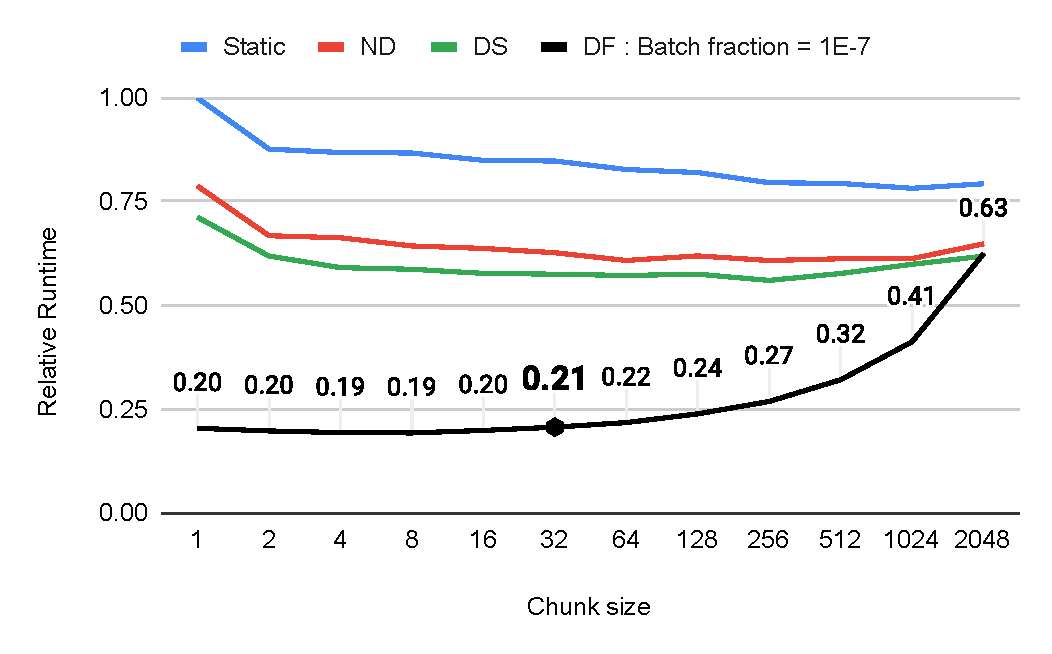
\includegraphics[width=0.98\linewidth]{out/aggregation-adjust-chunksize7.pdf}
  }
  \subfigure[Relative runtimes on uniformly random batch updates of size $10^{-5}|E|$]{
    \label{fig:aggregation-adjust-chunksize--batch5}
    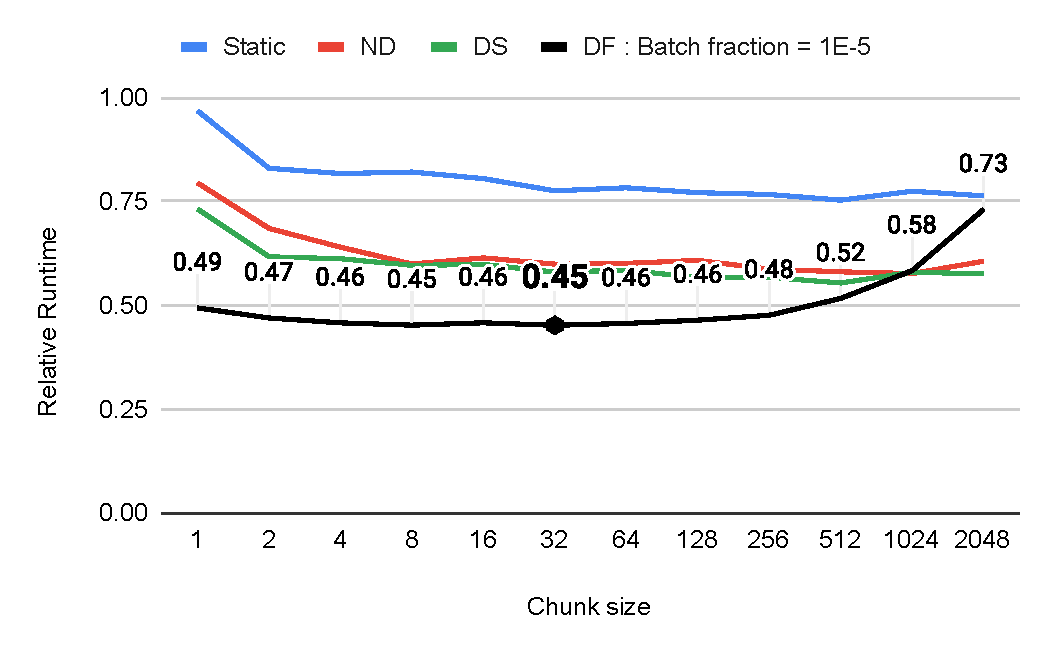
\includegraphics[width=0.98\linewidth]{out/aggregation-adjust-chunksize5.pdf}
  }
  \subfigure[Relative runtimes on uniformly random batch updates of size $10^{-3}|E|$]{
    \label{fig:aggregation-adjust-chunksize--batch3}
    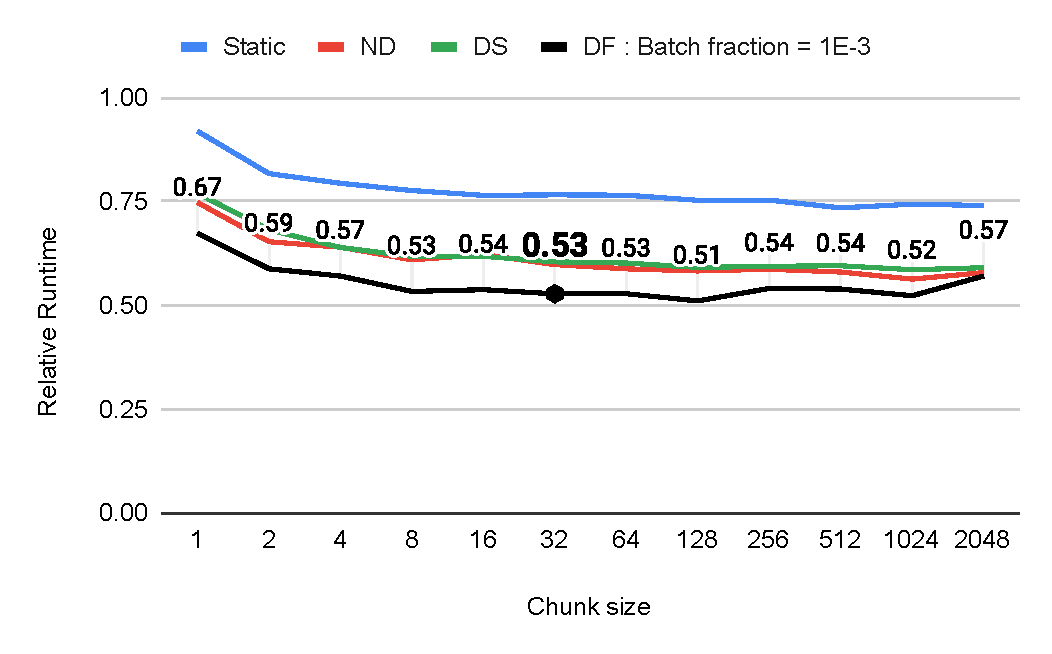
\includegraphics[width=0.98\linewidth]{out/aggregation-adjust-chunksize3.pdf}
  } \\[-1ex]
  \caption{Relative Runtime of \textit{Static}, \textit{Naive-dynamic (ND)}, \textit{Delta-screening (DS)}, and \textit{Dynamic Frontier (DF)} Leiden, with varying dynamic schedule chunk size (OpenMP), for aggregation phase of the Leiden algorithm. These tests were conducted on large graphs, with batch updates randomly generated at sizes of $10^{-7}|E|$, $10^{-5}|E|$, and $10^{-3}|E|$. The results suggest that a chunk size of $32$ is optimal (highlighted). In this figure, relative runtimes are normalized to maximum runtime, specifically that of Static Leiden with a chunk size of $1$ for dynamic scheduling during the aggregation phase.}
  \label{fig:aggregation-adjust-chunksize}
\end{figure}
